\ifpdf
\graphicspath{ {Chapters/Alignment/Figs/} }
\section{COMPASS Alignment}

\begin{frame}%[label=current]
  \frametitle{Alignment Motivation $\qquad \quad \color{red} \mathscr{RH} \text{
      contributions to analysis}$}

  \begin{itemize}
  \item COMPASS includes over 350 detector planes which need to be aligned
  \item Reconstructing particle tracks is not possible without
    alignment
  %\item Accomplished by minimizing a $\Chi^2$ function
  \item First check of spectrometer performance
  \end{itemize}

  \begin{columns}
    \column{0.48\textwidth}
    \begin{figure}
      \centering
      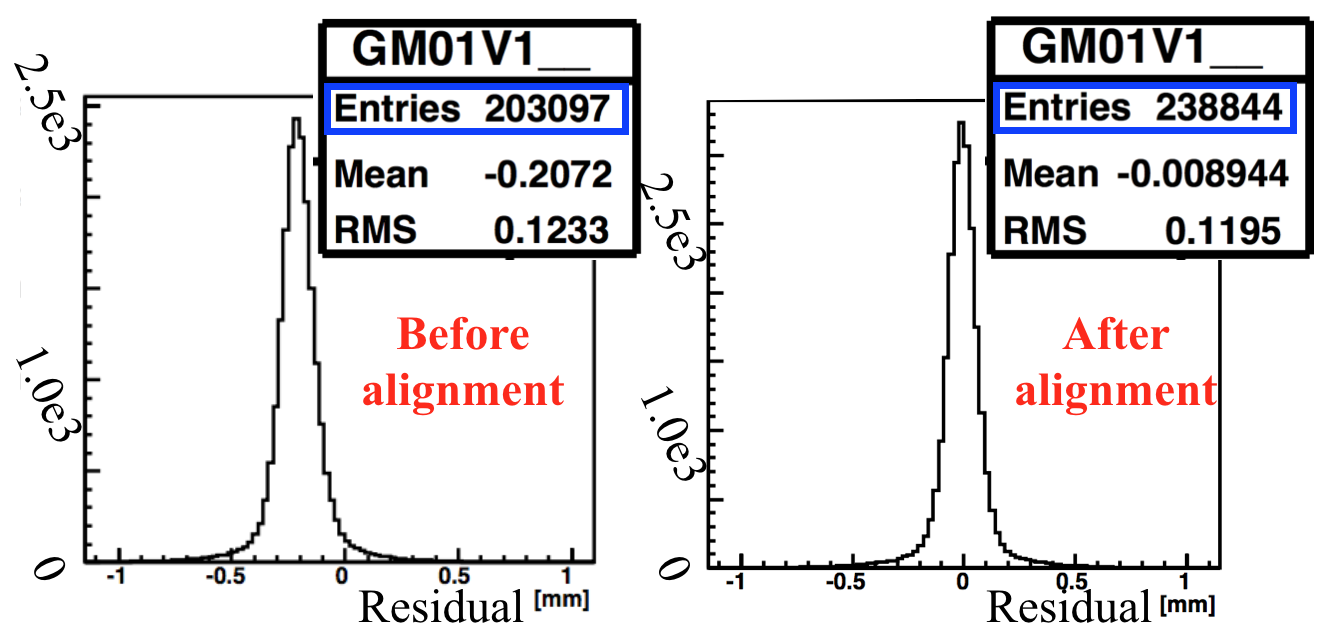
\includegraphics[width=\textwidth]{GMalign}
      \caption{Alignment effects, GEM type detector.}
    \end{figure}
    \column{0.5\textwidth}
    \begin{figure}
      \centering
      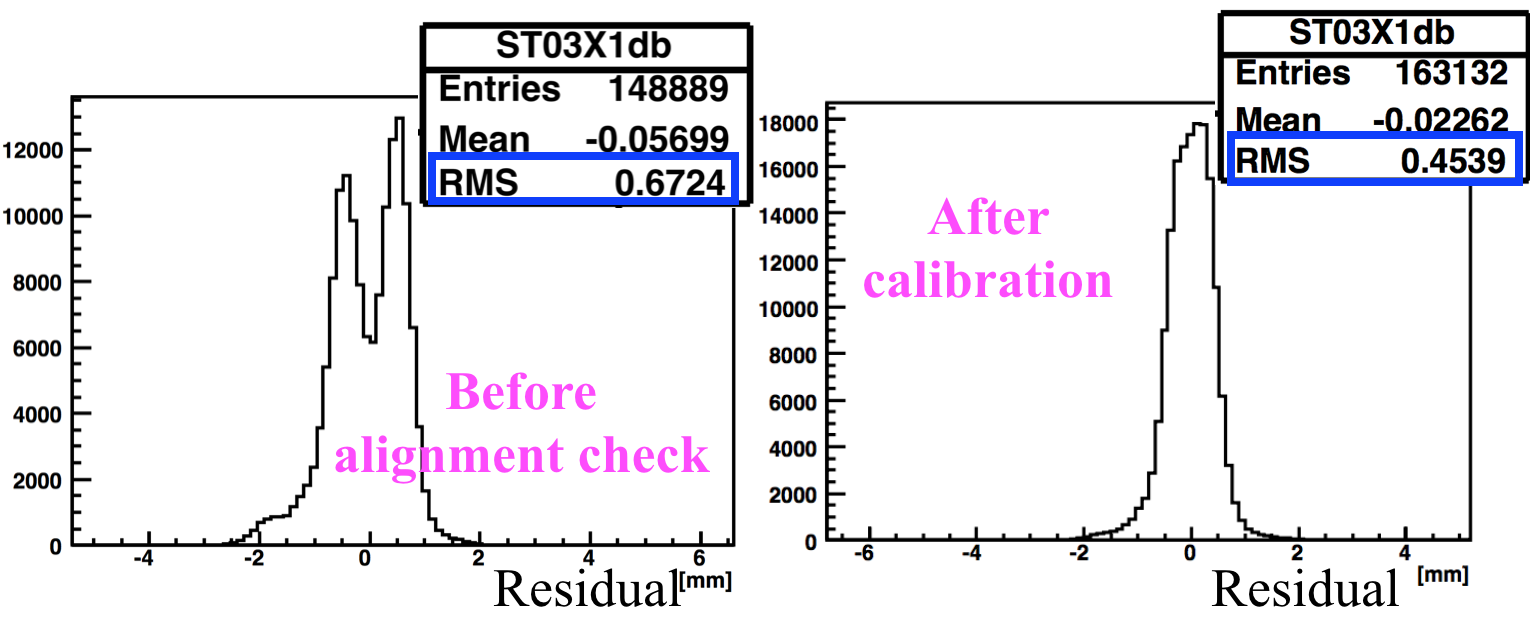
\includegraphics[width=\textwidth]{STalign}
      \caption{Calibration effects for straw type detector.}
    \end{figure}
  \end{columns}
\end{frame}


%\subsection{Alignment Data}
\begin{frame}
  \frametitle{Alignment Data}

  \begin{itemize}
  \item Low intensity alignment runs taken each data period
  \item $\mu^-$ beam used to have straight tracks
  \item Trigger system modified and detector centers turned on to
    maximally illuminate detectors
  \end{itemize}

  \begin{figure}
    \centering
    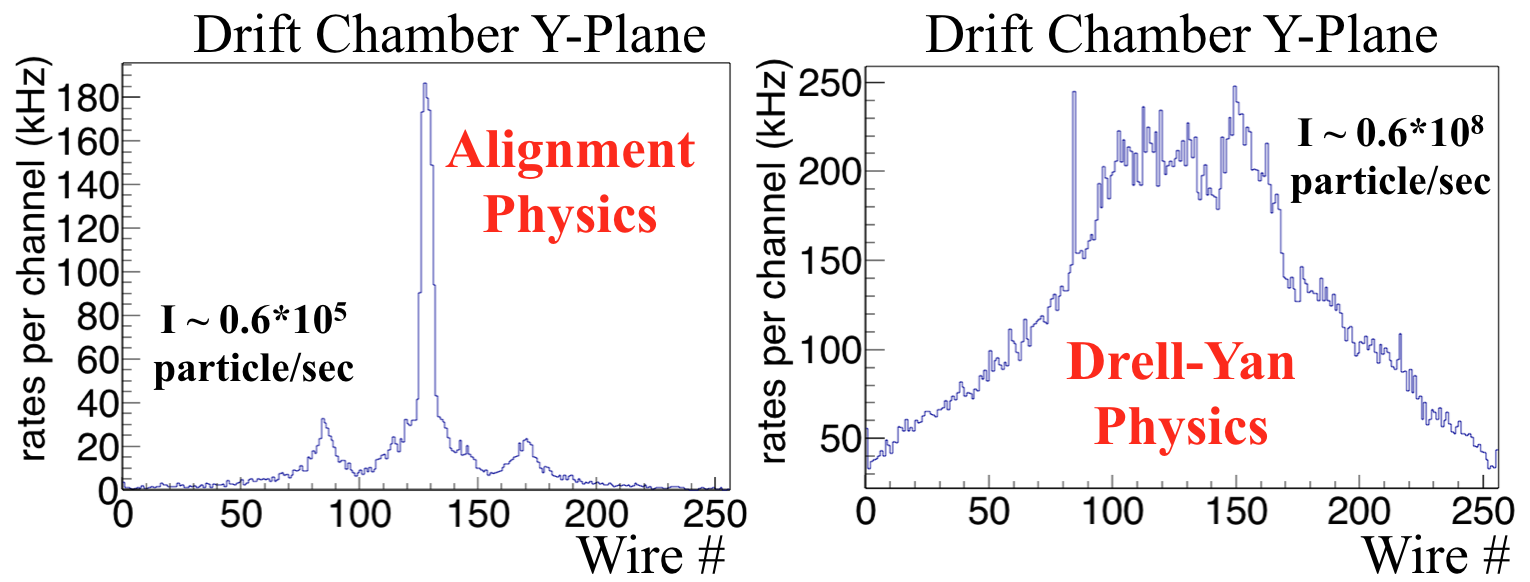
\includegraphics[width=\textwidth]{AlignmentRun}
    \caption{Detector data monitoring plots.}
  \end{figure}
\end{frame}


%\subsection{Alignment Procedure}
\begin{frame}%[label=current]
  \frametitle{Alignment Procedure Checks $\color{red} \mathscr{RH} \text{ contributions to analysis}$}
  
  \begin{itemize}
  \item Alignment performed by minimizing $\chi^2$ function of all
    track residuals
  \item Detectors aligned in 4 parameters:
    \begin{itemize}
    \item x position, y position, angle, wire/strip pitch
    \end{itemize}
    
  \item Alignment procedure iterated several times for best residuals
  \item 3 residual types checked to ensure alignment converged
  \end{itemize}

  \begin{figure}
    \centering
    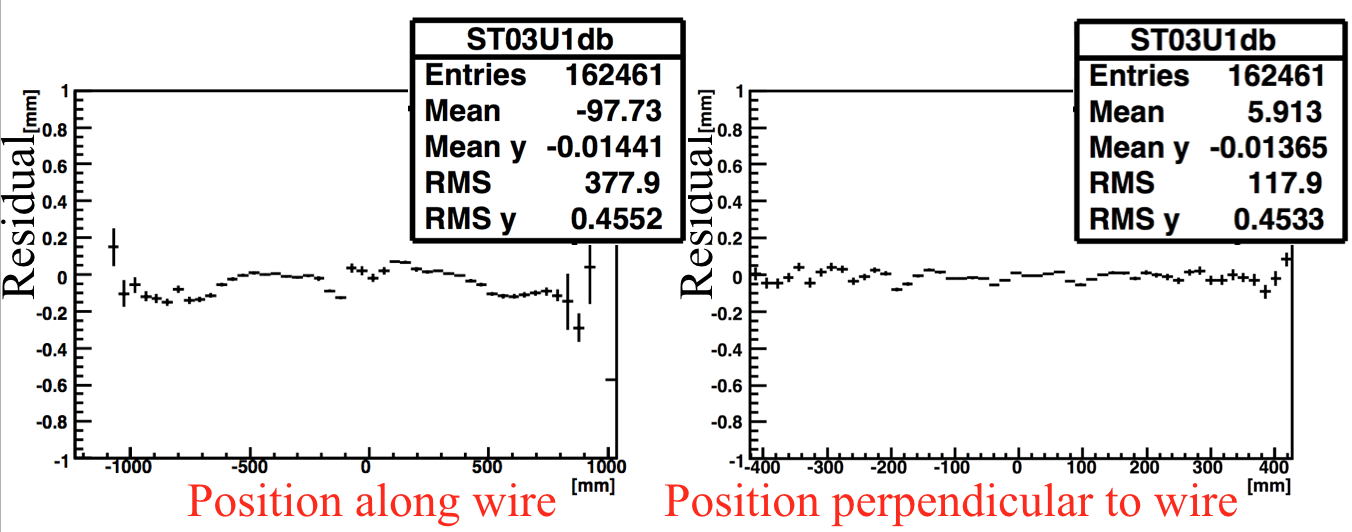
\includegraphics[width=\textwidth]{AlignmentChecks}
    %\caption{}
  \end{figure}
\end{frame}
